\section{Task 1 - Lexer}
\subsection{Explanation and Implementation}
The Lexer tokenizes the input stream by taking in character by character, grouping then into ordered tokens. A token is a tuple of (Lexeme, Attribute).

The following transition groups fo the characters were chosen (This is also the Classifier Table):
\begin{enumerate}
	\item Singular punctuation (punctuation which exists on its own): + - ( ) \textbraceleft \textbraceright ; $\colon$ ,
	\item Exclamation point: !
	\item Fullstop: .
	\item Digit: 0-9
	\item Alpha: A-Z a-z \textunderscore
	\item Forward slash: /
	\item New-line: \textbackslash n
	\item Asterisk: *
	\item Equals: =
	\item Whitespace/tab or \textbackslash r: ' ' \textbackslash t \textbackslash r
	\item Greater/Smaller than: \textless  \textgreater
	\item Other: anything else
\end{enumerate}

The following diagram is the state transition diagram DFA. Note: 'not X' means any other character which is not X.
\begin{figure}[H]
	\centering
	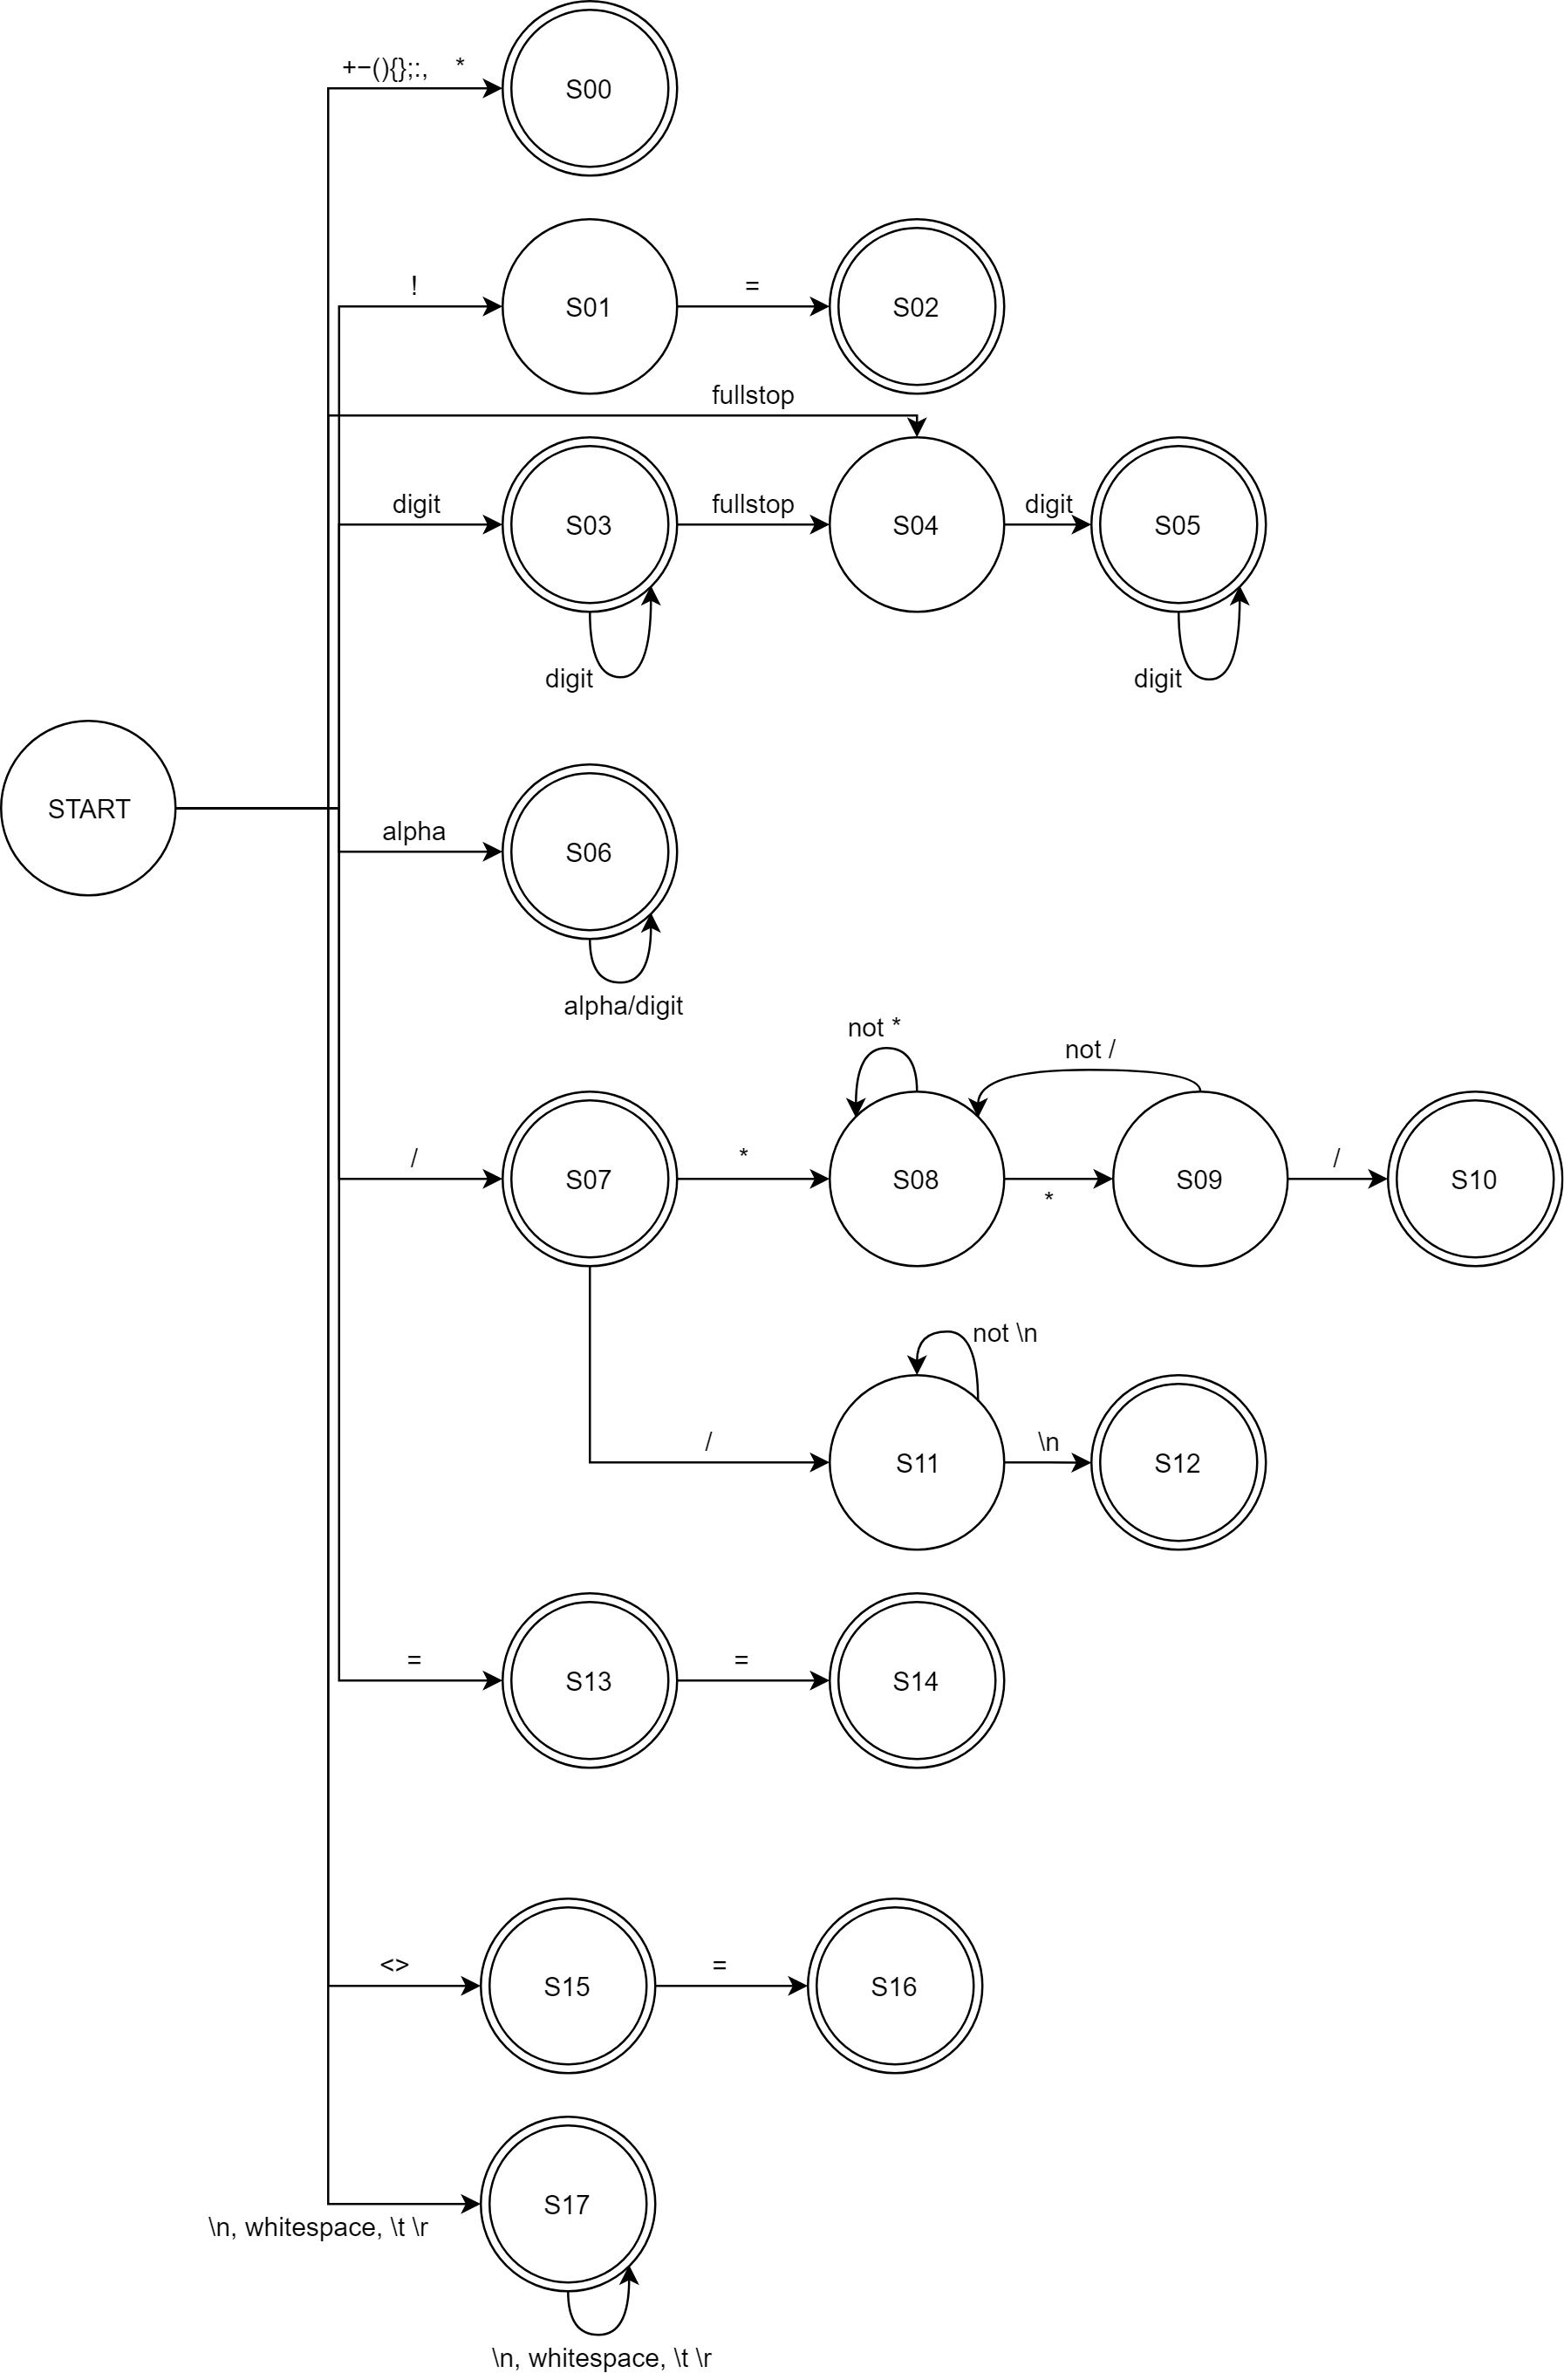
\includegraphics[scale=0.22]{Images/Q1_StateTransitionDiagram.png}
	\caption{DFA for Lexer}
\end{figure}

As a table, it looks like this in the code:
\begin{figure}[H]
	\centering
	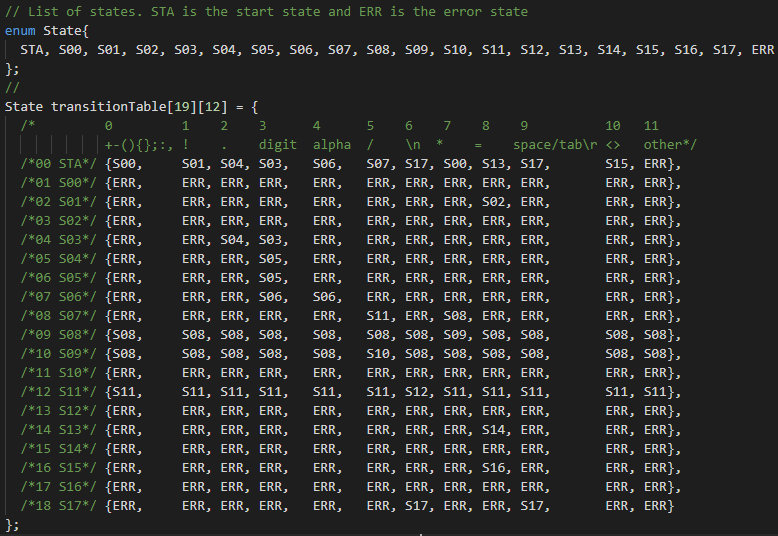
\includegraphics[width=\textwidth]{Images/Q1_StateTransitionTable.PNG}
	\caption{Table for Lexer}
\end{figure}

If the program goes to ERR (the error state), then the lexeme is over. If the current state is not a final state, then an error is reported and Lexical Analysis stops. If if the program goes to ERR and is in a final state, then the lexeme is kept and tokenized.

The token class is the following (Found in the Token.h file):
\begin{lstlisting}[language=C++]
class Token{
	public:
		static string TokenString[]; // Stings corresponding to the enum of token types
		enum TokenType{
		ID, BOOL, FLOAT, INT, // ID and constants
		ST, SE, GT, GE, EQQ, NE, AND, OR, NOT, // conditional operators
		EQ, PLUS, MINUS, TIMES, DIVISION, //arithmetic operators
		IF, ELSE, FOR, WHILE, FN, RETURN, TYPE_BOOL, TYPE_FLOAT, TYPE_INT, VAR, //keywords
		COLON, SEMI_COLON, COMMA, //punctuation
		OPEN_BRACKET, CLOSED_BRACKET, OPEN_BRACE, CLOSED_BRACE, //brackets punctuation
		COMMENT
		};
		
		// the Token parameters
		TokenType type;
		string lexeme = "";
		float number;
		
		// constructor
		Token (TokenType _type, string _lexeme, float _number){
		type = _type;
		lexeme = _lexeme;
		number = _number;
}

// helper method to neatly print the current token
void printToken();
};
\end{lstlisting}

The final states result in some token. The following is a list of which states can result to which tokens (based on the lexeme).
\begin{enumerate}
	\item S0: PLUS, OPEN\textunderscore BRACKET, CLOSED\textunderscore BRACKET, OPEN\textunderscore BRACE, CLOSED\textunderscore BRACE, COLON, SEMI\textunderscore COLON, COMMA, TIMES
	\item S2: NE
	\item S3: INT
	\item S5: FLOAT
	\item S6: ID (or one of mykeywords[] below)
	\item S7: DIVISION
	\item S11: discard '/*' and '*/' and return COMMENT
	\item S13: discard '//' and return COMMENT
	\item S14: EQ
	\item S15: EQQ
	\item S16: GT, ST
	\item S17: GE, SE
	\item S18: discard, since it is white spaces or new lines or tabs or carriage returns only
\end{enumerate}

\bigskip

The array of keywords in Token.cpp is as follows:
\begin{lstlisting} [language=C++]
// Used to check if a given string is a keyword (or identifier), and what type of keyword it is
struct keyword_token{
	string text;
	Token::TokenType tok_type;
};

keyword_token my_keywords[] = {
	{"and", Token::AND},
	{"or", Token::OR},
	{"not", Token::NOT},
	{"if", Token::IF},
	{"else", Token::ELSE},
	{"for", Token::FOR},
	{"while", Token::WHILE},
	{"fn", Token::FN},
	{"return", Token::RETURN},
	{"bool", Token::TYPE_BOOL},
	{"float", Token::TYPE_FLOAT},
	{"int", Token::TYPE_INT},
	{"var", Token::VAR},
	{"true", Token::BOOL},
	{"false", Token::BOOL}
};
\end{lstlisting}

\subsection{Example Test}
Using the \textit{printToken()} in the \textit{Token} class \textit{printTokens()} method in the \textit{Lexer} class, when the following input is given to the program:
\begin{lstlisting}
someid true false 12.3 .4 56 89
< <= > >= == != and or not
= + - * /
if else for while fn return bool float int var
: ; ,
() {}
// hello world
/* hello 
world
2 */
\end{lstlisting}
The following output is printed from \textit{printTokens()}

\begin{figure}[H]
	\centering
	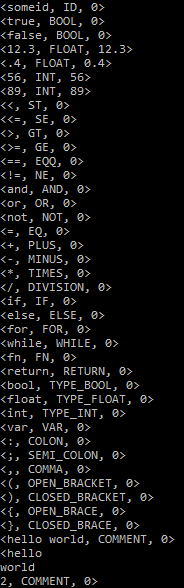
\includegraphics[scale=1]{Images/Q1_ExampleTest.png}
	\caption{Example output for the example input}
\end{figure}

